\chapter{Improving the Way Neural Networks Learn}


\begin{exercise}
Show that the cross-entropy function is minimized when $\sigma(z) = y$ for all inputs.
\end{exercise}
\begin{solution}
The cross-entropy function is defined as:
\[
    C = - \frac{1}{m} \sum_{i = 1}^m [y_i \ln (a_i) + (1 - y_i) \ln (1 - a_i)],
\]
where the $y_i$s are fixed and the $a_i$s are the ``variables.'' Now $\partial C / \partial a_i$
is given by:
\[
    \frac{\partial C}{\partial a_i} = \frac{1}{m} \frac{a_i - y_i}{a_i (1 - a_i)}. 
\]
At an extremum point of $C$, each component of the gradient $\nabla_a C$ will be zero. This 
happens when $a_i = y_i$ for all~$1 \leq i \leq m$. 

As a side note, the function $H(y) = - [y \ln(y) + (1 - y) \ln (1 - y)]$ for $y \in (0, 1)$ 
is called the binary entropy function and behaves as shown in Figure~\ref{fig:binary_entropy}. 
\end{solution}

\begin{figure}[ht]
\begin{center}
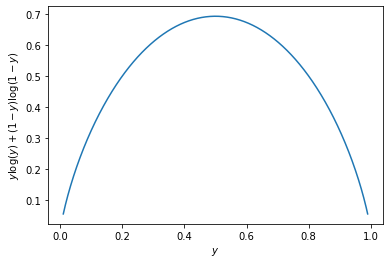
\includegraphics[scale=0.60]{entropy.png}
\end{center}
\caption{The Binary Entropy Function}
\label{fig:binary_entropy}
\end{figure}


